\chapter{What causes the Uncanny Valley?}
Soon after Masahiro Mori hypothesized the uncanny valley, the question what causes the uncanny valley arose. Viewed simply, there can only be two answers to this question. Either the uncanny valley has an evolutionary origin and therefore develops at a very young age or the uncanny valley arises through external influences over one's life experiences, therefore having a societal origin. 
\section{Explanatory hypotheses of the Uncanny Valley}
According to Strait et al. \cite{childrens_responding} there are two primary perceptually oriented hypotheses, which thus support the evolutionary origin of the Uncanny Valley: the category ambiguity hypothesis and the feature atypicality hypothesis.\\
The category ambiguity hypothesis \cite{childrens_responding} is based on the difficulty, for us humans, in categorizing very, but not completely human-like entities. This categorisation has evolved in the course of our evolution and is one of the
most basic human cognitive abilities. The valley-related discomfort is thus triggered when an entity cannot be categorised easily, which is the case at category boundaries as for example the robot-human boundary. The category ambiguity hypothesis may also suggest that the uncanny valley is unavoidable due to the automatic categorisation humans experience when looking at different entities.\\
The feature atypicality hypothesis \cite{childrens_responding} argues that the uncanny valley has it's origin in atypical features of figures that violate the expectations of their appearance or behaviour. An example of this would be a figure with a human-like head and a mechanical body. Such a figure would thus violate our expectations of how an actor should look like or behave. Therefore this theory proposes that overall consistency in regards to anthropomorphic or mechanomorphic features could avoid the Uncanny Valley effect.\\
The category ambiguity hypothesis and the feature atypicality hypothesis both explain the emergence of the uncanny valley through evolutionary processes. On the other hand, there is the theory that the uncanny valley arises through social influences over the course of a lifetime. Social triggers here could be, for example, the fear of humans being replaced by machines, which is spread by films or similar media. According to this theory, the uncanny valley would thus only develop with exposure to certain social influences and should therefore not be present at all or be less present in children or people who have been avoiding these social influences. 
\section{Differentiating between the Explanatory Hypotheses}
In order to find the origin of the uncanny valley, we must first distinguish between the opposing major theories. Is the uncanny valley caused by our perception and has therefore an evolutionary origin or by social influences? After a consensus has been found in existing studies, it is then possible to differentiate between either the two main hypotheses in the perceptually oriented direction, the category ambiguity hypothesis and the feature atypicality hypothesis, or between different influences that could cause the uncanny valley through social effects. Since social influences are only acquired over the course of time, children and infants should not yet have been influenced by them, which means that they should experience the uncanny valley effect less or not at all. The following discusses studies that have conducted experiments, testing whether the uncanny valley is already present in infants and children.
\subsection{Development of the Uncanny Valley in Infants}
A study by Lewkowicz et al. \cite{uncanny_infants} investigated the visual preferences of 6-, 8-, 10- and 12-month-old infants towards human faces, realistic avatar faces and uncanny avatar faces to understand the synergy of evolutionary and developmental influences on the maturing of the uncanny valley effect. For their experiment they choose 96 infants of mostly Caucasian phenotype and conducted three experiments in which they presented all possible pairs of three 6 pictures containing two human faces, two uncanny avatar faces and two realistic avatar faces, as seen in the figure \ref{fig:uncannyInfants}, to the infants. 
\begin{wrapfigure}[12]{r}{0.6\textwidth} %this figure will be at the right
    \centering
    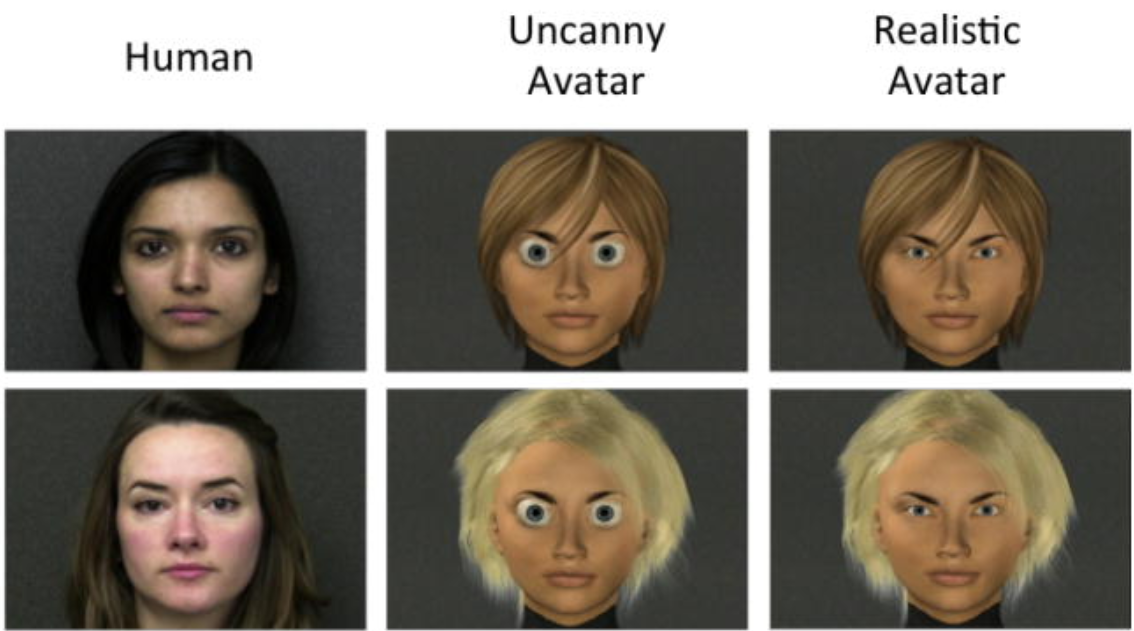
\includegraphics[width=0.6\textwidth]{graphics/uncanny_infants.png}
    \caption{Images of the three different types of faces.}
    \label{fig:uncannyInfants}
\end{wrapfigure}
In the first experiment the uncanny avatar faces were combined with the human faces to monitor the time the infants would look at the different faces. For the second experiment the uncanny avatar faces were paired with the realistic avatar faces. The main difference between the realistic and uncanny faces where the unrealistically large eyes of the uncanny faces. This experiment therefore tested mainly whether infants are sensitive to the large eyes by monitoring the time the infants looked at the different faces. In the third experiment the realistic avatar faces where combined with the human faces to test if the response of the first experiment would be based on the eye size or if the infants were more sensitive to how closely the faces resembled a human prototype.\\
The results of this study provide an interesting new insight into the uncanny valley effect. The first experiment showed a dramatic shift in infant response to the uncanny avatar faces and human faces depending on their age. The 6-month-old infants preferred the uncanny avatar face instead of the human face, while the 12-month-old infants preferred the human face instead of the uncanny avatar face. It can therefore be assumed that the Uncanny Valley effect is not yet present in the first six months of life but it develops during the second half of the first year.\\
The second experiment was able to confirm that the infants are highly sensitive to eye size differences and that they preferred the faces with normal sized eyes.\\
The results of the third experiment verified that the infants mainly paid attention to the eyes and did not recognise the synthetic nature of the realistic character. This further proved the main finding of the study that infants looked less at the uncanny avatar because of the unusual large eyes.\\
In summary, this study suggests an interplay between the early influences on infant development and evolutionary mechanisms as the cause of the uncanny valley. Once infants have learned the prototype they likely have sufficient perceptual experience to recognise irregularities in imperfect humanlike entities, which then triggers the uncanny valley. It is also clear from previous studies that perceptual abilities are relatively crude at the start of life, but improve rapidly during the first year \cite{Lewkowicz2009_perceptual_abilities,Pascalis2009_perceptual_abilities}. Specific developmental experiences of faces and emotion let their observers quickly learn to recognise abnormalities and aesthetic values of a face. As a result, faces that are abnormal/not humanlike have a repulsive effect which causes an uncanny valley effect.\\\\
Matsuda et al. \cite{uncanny_infant_discrimination} conducted a very similar study testing the discrimination of infants against humanoid robots. In the study an experiment showing three different types of agents to 42 infants aged between 6 to 14 months was conducted. The chosen visual stimuli consisted of three different black and white video clips, which pictured a human, an android and a mechanical robot performing a grasping action with their right hand as shown in the figure \ref{fig:uncannyInfantsDiscrimination}. The infants were each shown two different videos of the agents which were played side by side. 
\newpage
The videos were paired into human and android, human and robot and android and robot combinations. Each of these pairs was shown to the infants four times for 10.5 seconds. During the experiment, the children were sitting on their parents' laps, who were instructed not to react either to the shown agents or to the infants. In order to analyse how the infants react to the different agents, their eye movements were monitored in real time.
\begin{wrapfigure}{r}{0.6\textwidth} %this figure will be at the right
    \centering
    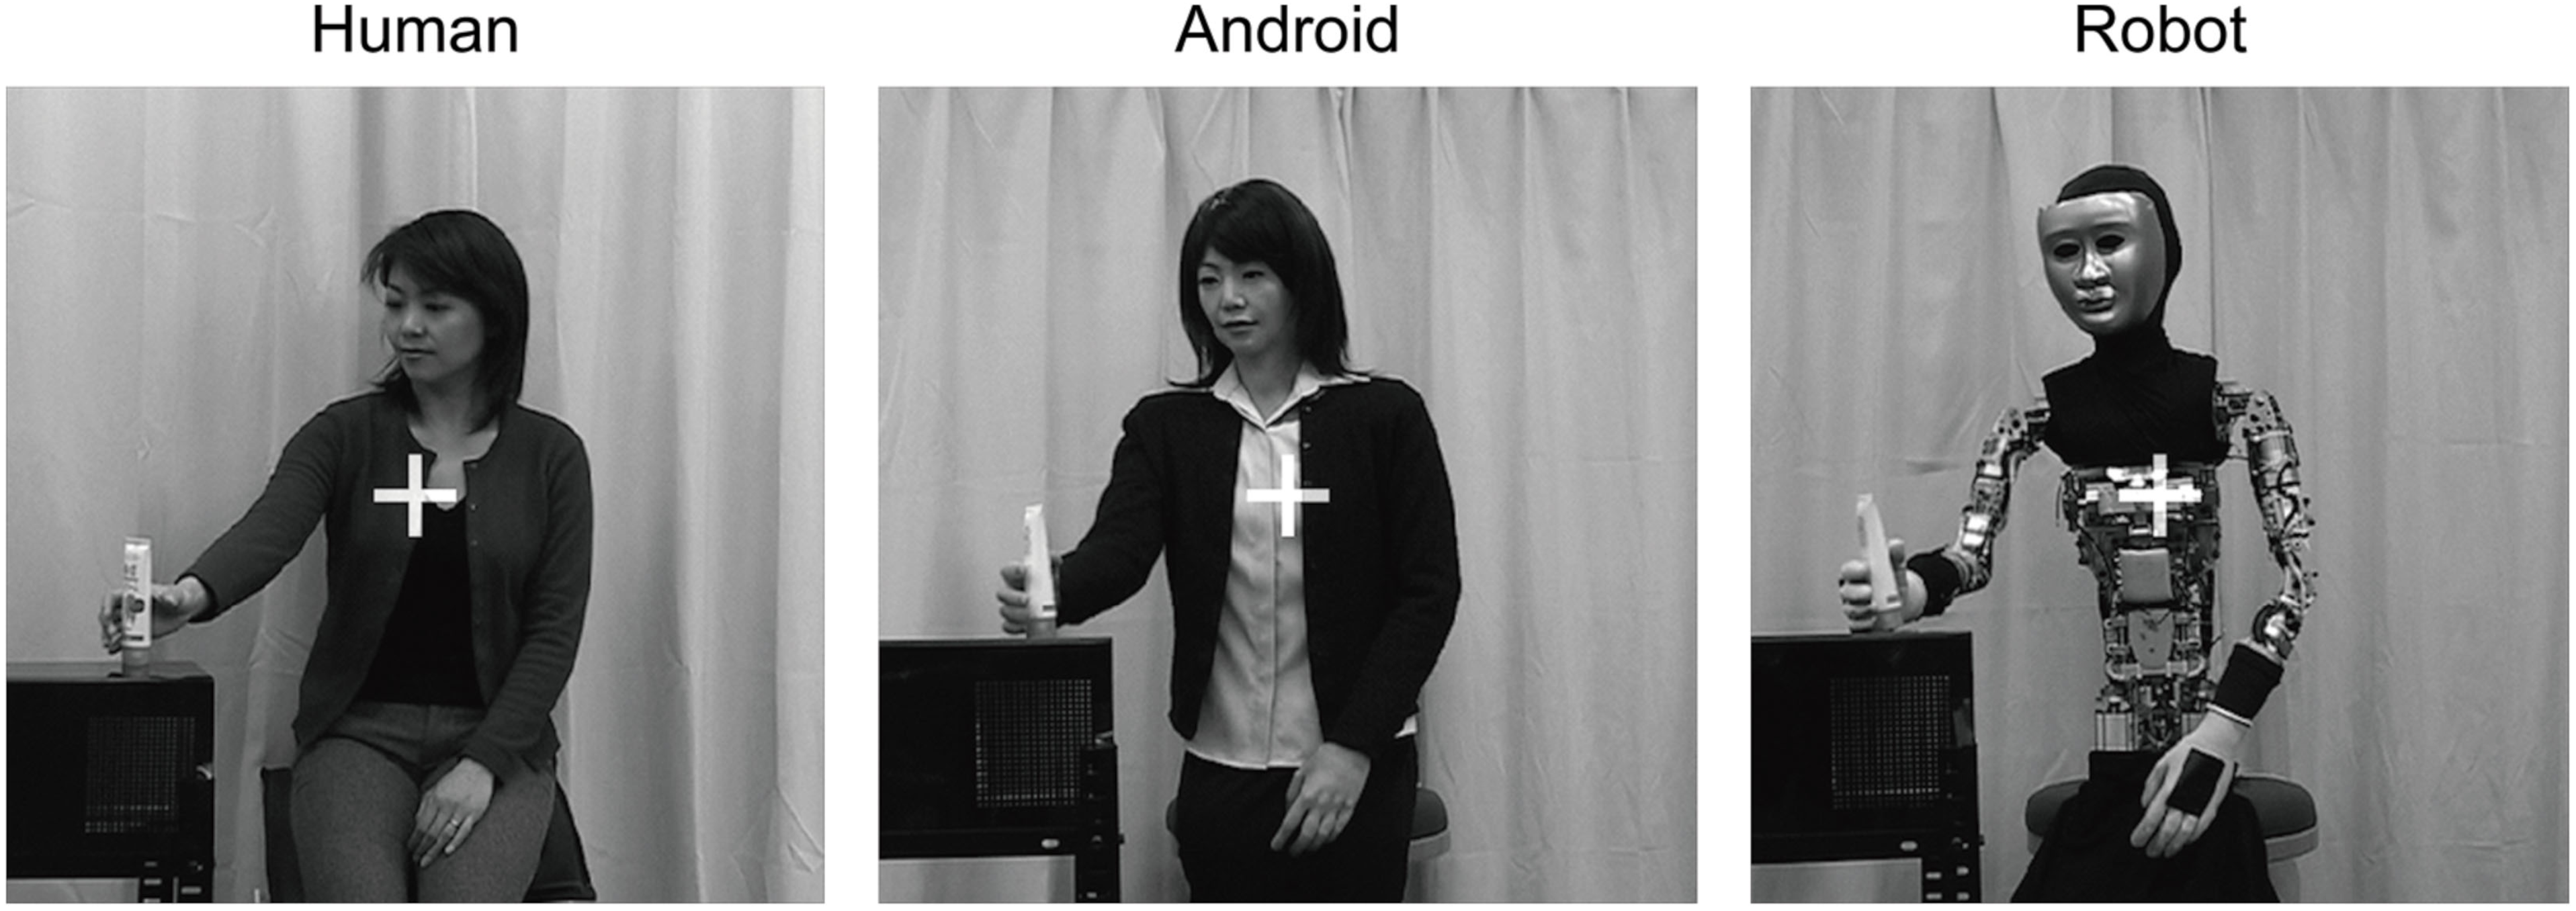
\includegraphics[width=0.6\textwidth]{graphics/uncanny_infants_discrimination.png}
    \caption{Images of the three different types of agents used.}
    \label{fig:uncannyInfantsDiscrimination}
\end{wrapfigure}
The results of the experiment show that the infants spent the longest time on viewing the robot. In contrast to studies conducted with adults, there was no difference in the viewing time between the human and android agents. So this study suggests that infants up to 14 months of age do not yet have the perceptual abilities to distinguish between the human and android looking agents. However, it seems that they are already able to distinguish humans from robots. Since infants have a tendency to observe novel objects, this could be a possible reason why they looked at the robots longer. In summary, this study did not find a discrimination against androids in infants. From the results of the study it can be suggested that the perceptual abilities of the infants were not yet well enough developed to recognize the subtle differences between the human and android agent. As a result, the infants had not yet developed an uncanny valley effect.\\\\
When comparing the two studies, one can see certain similarities but also disagreements. The study by Lewkowicz et al. \cite{uncanny_infants} proposes that infants would learn the necessary perceptual abilities gradually in their second half of their first year of life to differentiate between human agents and humanlike android agents. In contrast the the study by Matsuda et al. \cite{uncanny_infant_discrimination} could not find evidence that the infants aged 14 months could differentiate sufficiently between the android agents and the human agents. However they could already distinguish between humans and robots. By looking at the characters used by Lewkowicz et al. and Matsuda et al. one can see that the differences in the study by Matsuda et al. between the human and the uncanny agent are very subtle. On the contrary, the uncanny avatar from the study by Lewkowicz et al.  can be very easily be distinguished from the human face. This may be the reason for the lack of response from the infants to the android agents in the study by Matsuda et al. . Concluding, it seems that the development of the uncanny valley goes hand in hand with the development of perceptual abilities in infants. This development seems to occur between the 6 and 14 months of an infant's life, but the full development of these skills  may of course depend on the individual's developmental rate. This may explain the different results of the two studies. 
\newpage

\subsection{Observing the Uncanny Valley in Children}





